\section{Semantic Analysis}

\subsection{Phases \& Design}

As described in \ref{eyecandy} the Semantic Analysis phase
should be split into a number of sub-phases specifically: symbol
resolution, de-sugaring/type inference and type checking.

However, these steps can be combined together into a single step
phase. There a benefits and downsides to both approaches. The
main benefit of using the first approach is a reduction in
algorithmic complexity. The logic can be separated into
different phases with ease and information from one phase can be
propagated to another. The downside of this approach is that it
actually adds more code for maintenance, since each individual
sub-phase will probably need to be implemented as its own
visitor. The other down side is error management. If an error
occurs in a particular phase since said phase is completely
disjoint from the phases after it a mechanism for propagation
needs to be devised which again further increases complexity. Of
course by the very nature of this argument the monolithic
approach does not suffer for the issues that the sub-phases
approach has. However, it significantly increases complexity
since all sub-phases are being done in a single phase. The other
more glaring issue is the fact that it is much more difficult to
resolve symbols before-hand.

You would want to do so to allow for the location of function
declarations in code to not effect resolution, that is, a
function can be called before it is referenced.

Unfortunately, due to the fact that compiler development was an
organic process and not too much time was spend on deliberation
the semantic analysis phase became monolithic, and hence it
suffers from the issues described above. Of course, this means
location agnostic function declaration are currently \emph{not}
supported by the compiler.

\subsection{The Environment Tree}

Some terminology is required to properly describe the number of
structures which will be used in this section. The following
terms are critical and need to be differentiated properly:

\begin{itemize}
    \item \texttt{SymbolTable}
    \item \texttt{SymbolTableStack}
    \item \texttt{Environment}
    \item \texttt{EnvStack}
    \item \texttt{RefStack}
\end{itemize}

During semantic analysis there is the need for specific data
structures which facilitate scoping rules, type checking, etc.

The most basic form of this is a single \texttt{SymbolTable}. A
symbol table in its simplest form is a wrapper around a hash
map. Of course this is quite a limiting structure. In the
context of a full program usage of such a structure for semantic
analysis will restrict the users of the language to be careful
regarding their naming as everything in the language would be in
global scope.

Therefore, this is not even a sufficient solution for most
toy-languages let alone full-blown production ready languages.
The solution to this problem is the use of a stack of symbol
tables. This allows symbol tables to shadow each other allowing
for the reuse of names. Additionally, this further opens up the
possibility of implementing language level modules. The
likelyhood that names will be reused across different modules is
quite high and being able to scope modules so they do not
interfere with global scope allows multiple modules and the main
executable to co-exist.

\begin{figure}[H]
\centering
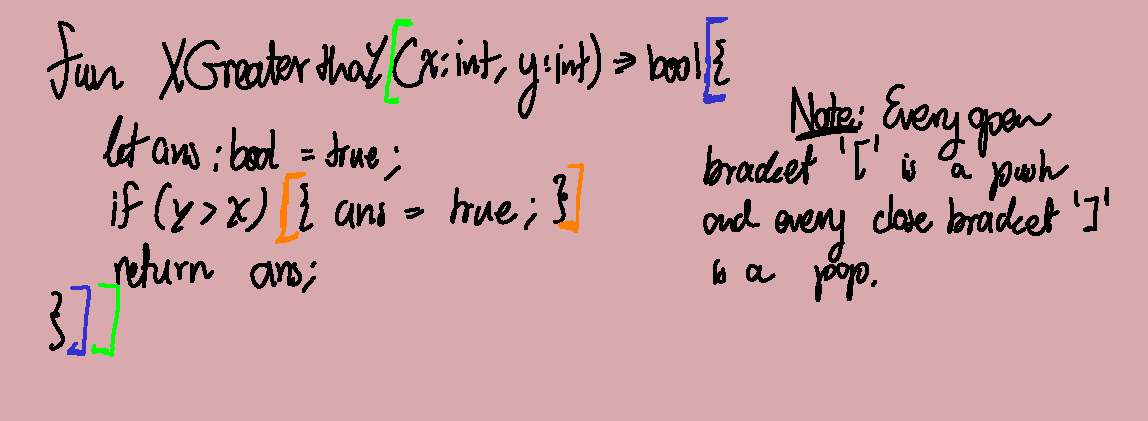
\includegraphics[width=\linewidth]{scopedcode.pdf}
\caption{A \texttt{PArL} function with annotated scopes}
\label{fig:scopeannotatedcode}
\end{figure}

The basic premise of using a symbol table stack is described
in

\begin{algorithm}[H]
    \KwData{$N$ the AST node, $S$ the \texttt{SymbolTableStack}}
\Begin{
$V \longleftarrow U$\;
$S \longleftarrow \emptyset$\;
\For{$x\in X$}{
$NbSuccInS(x) \longleftarrow 0$\;
$NbPredInMin(x) \longleftarrow 0$\;
$NbPredNotInMin(x) \longleftarrow |ImPred(x)|$\;
}
\For{$x \in X$}{
\If{$NbPredInMin(x) = 0$ {\bfseries and} $NbPredNotInMin(x) = 0$}{
$AppendToMin(x)$}
}
\nl\While{$S \neq \emptyset$}{\label{InRes1}
\nlset{REM} remove $x$ from the list of $T$ of maximal index\;\label{InResR}
\lnl{InRes2}\While{$|S \cap ImSucc(x)| \neq |S|$}{
\For{$ y \in S-ImSucc(x)$}{
\{ remove from $V$ all the arcs $zy$ : \}\;
\For{$z \in ImPred(y) \cap Min$}{
remove the arc $zy$ from $V$\;
$NbSuccInS(z) \longleftarrow NbSuccInS(z) - 1$\;
move $z$ in $T$ to the list preceding its present list\;
\{i.e. If $z \in T[k]$, move $z$ from $T[k]$ to
$T[k-1]$\}\;
}
$NbPredInMin(y) \longleftarrow 0$\;
$NbPredNotInMin(y) \longleftarrow 0$\;
$S \longleftarrow S - \{y\}$\;
$AppendToMin(y)$\;
}
}
$RemoveFromMin(x)$\;
}
}
\caption{Basic description of \texttt{SymbolTableStack} usage}
\end{algorithm}

\begin{figure}[H]
\centering
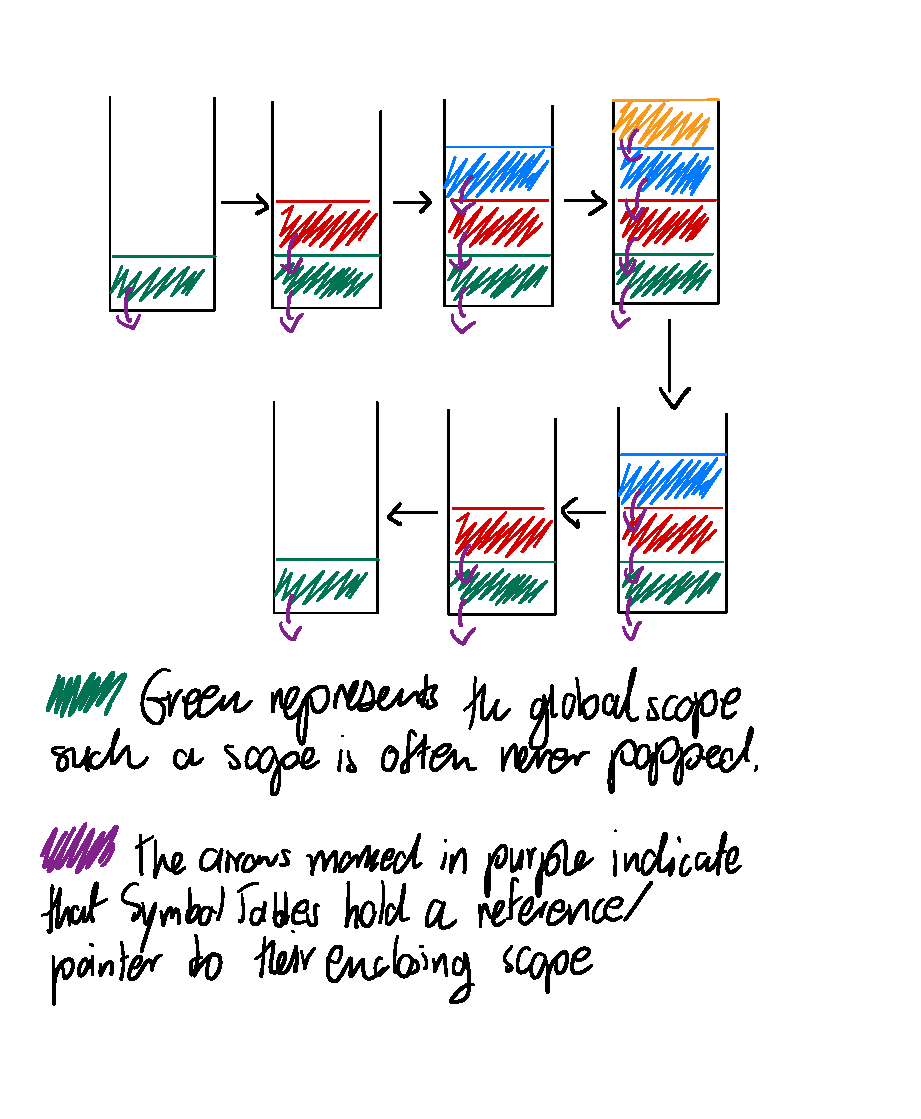
\includegraphics[width=\linewidth]{symboltablestack.pdf}
\caption{Behaviour of the \texttt{SymbolTableStack} when
considering the code in \figref{scopeannotatedcode}}
\end{figure}


Arguably the most important part of the later stages of
a compilation is the Environment tree.

The Environment tree is a data structure

\begin{itemize}
    \item Describe Symbol Table.
    \item Describe each element of the symbol table.
    \item Describe the tree approach.
    \item attribute the tree approach to Robert Nystrom as well.
    \item describe the main advantage/disadvantage of using a environment
        approach.
    \item describe the main advantage/disadvantage of using a symbol stack
        approach.
\end{itemize}
